% This is "sig-alternate.tex" V2.0 May 2012
% This file should be compiled with V2.5 of "sig-alternate.cls" May 2012
%
% This example file demonstrates the use of the 'sig-alternate.cls'
% V2.5 LaTeX2e document class file. It is for those submitting
% articles to ACM Conference Proceedings WHO DO NOT WISH TO
% STRICTLY ADHERE TO THE SIGS (PUBS-BOARD-ENDORSED) STYLE.
% The 'sig-alternate.cls' file will produce a similar-looking,
% albeit, 'tighter' paper resulting in, invariably, fewer pages.
%
% ----------------------------------------------------------------------------------------------------------------
% This .tex file (and associated .cls V2.5) produces:
%       1) The Permission Statement
%       2) The Conference (location) Info information
%       3) The Copyright Line with ACM data
%       4) NO page numbers
%
% as against the acm_proc_article-sp.cls file which
% DOES NOT produce 1) thru' 3) above.
%
% Using 'sig-alternate.cls' you have control, however, from within
% the source .tex file, over both the CopyrightYear
% (defaulted to 200X) and the ACM Copyright Data
% (defaulted to X-XXXXX-XX-X/XX/XX).
% e.g.
% \CopyrightYear{2007} will cause 2007 to appear in the copyright line.
% \crdata{0-12345-67-8/90/12} will cause 0-12345-67-8/90/12 to appear in the copyright line.
%
% ---------------------------------------------------------------------------------------------------------------
% This .tex source is an example which *does* use
% the .bib file (from which the .bbl file % is produced).
% REMEMBER HOWEVER: After having produced the .bbl file,
% and prior to final submission, you *NEED* to 'insert'
% your .bbl file into your source .tex file so as to provide
% ONE 'self-contained' source file.
%
% ================= IF YOU HAVE QUESTIONS =======================
% Questions regarding the SIGS styles, SIGS policies and
% procedures, Conferences etc. should be sent to
% Adrienne Griscti (griscti@acm.org)
%
% Technical questions _only_ to
% Gerald Murray (murray@hq.acm.org)
% ===============================================================
%
% For tracking purposes - this is V2.0 - May 2012

\documentclass{sig-alternate}

\begin{document}
%
% --- Author Metadata here ---
%\conferenceinfo{WOODSTOCK}{'97 El Paso, Texas USA}
%\CopyrightYear{2007} % Allows default copyright year (20XX) to be over-ridden - IF NEED BE.
%\crdata{0-12345-67-8/90/01}  % Allows default copyright data (0-89791-88-6/97/05) to be over-ridden - IF NEED BE.
% --- End of Author Metadata ---

\title{Writing A Security Protocol On Top of NFC}
%\subtitle{[Extended Abstract]
%  \titlenote{A full version of this paper is available as
%    \textit{Author's Guide to Preparing ACM SIG Proceedings Using
%      \LaTeX$2_\epsilon$\ and BibTeX} at
%    \texttt{www.acm.org/eaddress.htm}
%  }
%}
%
% You need the command \numberofauthors to handle the 'placement
% and alignment' of the authors beneath the title.
%
% For aesthetic reasons, we recommend 'three authors at a time'
% i.e. three 'name/affiliation blocks' be placed beneath the title.
%
% NOTE: You are NOT restricted in how many 'rows' of
% "name/affiliations" may appear. We just ask that you restrict
% the number of 'columns' to three.
%
% Because of the available 'opening page real-estate'
% we ask you to refrain from putting more than six authors
% (two rows with three columns) beneath the article title.
% More than six makes the first-page appear very cluttered indeed.
%
% Use the \alignauthor commands to handle the names
% and affiliations for an 'aesthetic maximum' of six authors.
% Add names, affiliations, addresses for
% the seventh etc. author(s) as the argument for the
% \additionalauthors command.
% These 'additional authors' will be output/set for you
% without further effort on your part as the last section in
% the body of your article BEFORE References or any Appendices.

\numberofauthors{2} %  in this sample file, there are a *total*
% of EIGHT authors. SIX appear on the 'first-page' (for formatting
% reasons) and the remaining two appear in the \additionalauthors section.
%
\author{
% You can go ahead and credit any number of authors here,
% e.g. one 'row of three' or two rows (consisting of one row of three
% and a second row of one, two or three).
%
% The command \alignauthor (no curly braces needed) should
% precede each author name, affiliation/snail-mail address and
% e-mail address. Additionally, tag each line of
% affiliation/address with \affaddr, and tag the
% e-mail address with \email.
%
  \alignauthor{Andrey Tydnyuk\\
  \affaddr{Carnegie Mellon University}\\
  \email{ait@andrew.cmu.edu}
  }
  \alignauthor{Srinivasan Seshan\\
  \affaddr{Carnegie Mellon University}\\
  \email{srini@cmu.edu}
  }
}

\maketitle
\begin{abstract}

Near Field Communication technology, or NFC as it is commonly called,
is a wireless radio communication standard that can be used to
exchange information between a device and a tag at close range. It is
a lot like RFID, but where RFID tags can be scanned at a distance of
meters, NFC tags need to be scanned at a distance of centimeters. The
upshot of this is that NFC allows two-way communication as opposed to
RFID tags that generally only support reading from the
tag\footnote{Newer RFID tags actually allow writing, but this is new
  and experimental}.

In this paper we explore the possibility of adding a security protocol
to NFC tags to allow secure location confirmation. For example, if a
restaurant wants to make sure that only people that have been to it
can submit reviews, it can place an NFC tag at the entrance/exit and
confirm that customers have scanned the tag before they are allowed to
submit a review online. We explore several different tag-device setups
under several attack scenarios. We show that it is possible to develop
a secure protocol with an on-phone TPM and a dumb tag that does not do
computation. If we relax the TPM requirement, we can have a ``good
enough'' solution that relies on the fact that only a certain fraction
of users are malicious.
\end{abstract}

% A category with the (minimum) three required fields
\category{H.4}{Mobile Systems Applications}{NFC, Security, Wireless}

\terms{Security, Reliability}

\keywords{NFC, Wireless, Security, TPM, Location Services, Simulation}

\section{Introduction}
NFC tag usage has been increasing since their mass production
release. Tags are pretty cheap and versatile. Some popular uses of
tags are to do location services such as checking in to places, or to
change phone settings based on pre-defined rules. Some examples of the
former are tags that are put up in front of restaurants or other
commercial places that give you a code to a website to confirm that
you have visited their location. This can be tied into different perks
for the user such as discounts or sales. NFC tags can also be used for
games or competitions that involve real-world locations. This can
range from scavenger hunts that depend on the user scanning tags to
get clues to games that assign territory based on number of visits to
a particular location.

All of these uses rely on the fact that there won't be truly malicious
users. Tolerating a few fake requests submitted through the web,
without ever visiting the tag is fine, but being protected against DOS
and other attacks is another. If the NFC tag associated with the
service supports writing, then a malicious user can write a different
clue or password or URL to the tag and thereby deny service or worse,
redirect service to his own malicious page. The only way to fix this
is for someone in charge to visit the site and write the correct
password back to the tag. This requires a human intervention for every
malicious user, and is not a reasonable solution.

On the other hand, if we disable writing and use a read-only tag we
have a scenario where the password never changes. If the password
never changes it can be put up online and accessed by anyone. While
this might not be a worry for a local scavenger hunt that operates
under an honor system, a review service operating in this scenario is
rendered completely useless. If the tag was put in place to make sure
that the reviews written are by actual past customers, the fact that
you can put the password up online and get multiple uses out of it
voids that guarantee.

In light of these difficulties we present several different systems
for dealing with attacks against an NFC tag based service. The
protocols and assumptions may differ for each setup, but there are
several commonalities. Each setup consists of three parts. There is a
tag that is located at a specific location that we want to securely
transmit, there is a device (phone) that will be scanning the tag, and
there is a webserver that will keep track of all of the scans and be
in charge of accepting or rejecting requests.

We start our analysis by detailing several different attack
models. Since there are a lot of attacks that can be done against this
kind of service we cannot cover all of them, but we list what we
believe to be the easiest to execute and the most debilitating for the
service itself. We will briefly mention other attacks that we did not
consider in our analysis and give reasoning for our choice.

After going over the different attacks we consider two different
setups to protect our service. The first setup assumes an on-phone TPM
that can be used to shield the user from accessing certain
information. This setup is found to be very effective at preventing
malicious users from affecting the service. With our protocol we
manage to prevent all but one of the attacks that we detailed in the
previous section and we do not drop any requests from honest
users. This is the best possible result, but it requires an on-phone
TPM which isn't something that is commercially available.

For the second setup, we relax the on-phone TPM requirement and
consider the lowest cost case of an average phone with NFC
reading/writing capabilities and a dumb tag that cannot do any
computation. In this case, we find that the protocol is vulnerable to
several attacks. Our solution to alleviate this problem is the
addition of a reputation system. We propose that the website keep a
reputation record for each user and show that this approach helps us
keep malicious users out of the system with minimal impact to honest
users as long as the the number of malicious users is about a tenth of
the number of honest users.

At the end of the paper we go over some opportunities for further
work.

\section{Attack Models}
In this section we will consider the different attacks that our
service will have to deal with. We will consider attacks in order
based on the ease of execution.

\subsection{Bogus Submissions}
Since the webserver is in charge of seperating the valid requests from
the invalid ones, the easiest attack to execute is to send bogus
requests to the webserver. This does not require ever being next to
the tag and can be done by anyone from the comfort of their own
house. 

The attack model that we consider for this is a maximum of 1 request
per second. While it might seem strange that we assume such a low
rate, especially considering that scripts can pump out hundreds of
requests per second from a single machine, dealing with DDOS is out of
the scope of this paper. Since there is no way a legitimate user can
scan more than one tag per second, it seems reasonable to limit the
number of requests that can come from a single IP to one per second.

\subsection{Publicizing the Password}
This attack is arguably simpler than the last one mentioned, but it
requires going to the actual location of the tag and scanning it. Once
the tag is scanned, the content of the tag is put up online for anyone
to access.

The attack model for this is fairly simple as well. Since you actually
need one person to go to the location, this attack is only harmful if
the password has multiple uses. If it doesn't, this attack falls under
another category that we will detail later.

\subsection{Multiple Scan}
This attack also involves a malicious user going to the location, but
this time instead of just scanning the tag once, the user scans the
tag multiple times. He then potentially walks away with several
passwords that he can distribute online at will.

For this attack, we accept that the passwords may be single-use, but
the attacker can scan the tag an unlimited number of times if
necessary and put the list up online. This way we get a similar effect
to the \texttt{Publicized Password} attack, with the additional
limitation that it takes more time for the user to stand and scan the
tag several times. Since malicious users don't really need a reason to
be malicious, we don't really regard it as a real limitation and just
assume that there will be someone who is willing to stand at the tag
for hours recording thousands of passwords.

\subsection{Tag Modification}
This is also an attack that involves a malicious user going to the
location of the tag. In this scenario, the user writes garbage or
malicious data to the tag. 

For this attack we assume that the attacker can write anything to the
tag and the frequency with which this happens is proportionate to the
number of malicious users in the system. We assume that this kind of
attack does not happen that often due to the requirement that the
malicious user has to be in range of the tag itself.

\subsection{Man in the Middle}
This attack requires the most effort on the attacker's part, and is
also the most difficult to defend against. This attack involves an
attacker scanning the tag, and instead of submitting the password,
forwarding it to a friend. The rest of the protocol proceeds a fashion
such that all communication between phone and webserver goes through
the middleman that is pretending to be at the tag location.

\subsection{Other Attacks}
We never cover snooping attacks for the simple reason that NFC
communication operates at a close range, so it is difficult to snoop
on a communication between a phone and a tag without being painfully
obvious to the honest user. We also never consider attacks on other
layers of the network stack because that is out of the scope of this
paper.

\section{Protocol 1: Phone with TPM + Dumb Tag}

\subsection{Outline}
This is a quick rundown of the protocol:

\begin{enumerate}
\item The device reads the tag and the tag sends the device a code, $k$
\item The key, $k$, goes into sealed storage
\item The device sends the phone IMEI and $k$ to the webserver
\item The webserver checks $k$ against the key that it is expecting
\item The key matches so the webserver generates the next key, $l$, to write to the tag
\item The webserver records the fact that the device's request was accepted
\item The ACCEPTED message and $l$ are sent to the device 
\item The device writes $l$ to the tag so the next person can use it
\end{enumerate}

That was a step by step overview of what happens when an honest user
uses the protocol. The interesting stuff happens when malicious users
enter the picture. For a comprehensive look at this we need to look at
the different states that the protocol can be in depending on what
requests it gets.

\subsection{Protocol States}
\begin{figure}
\centering
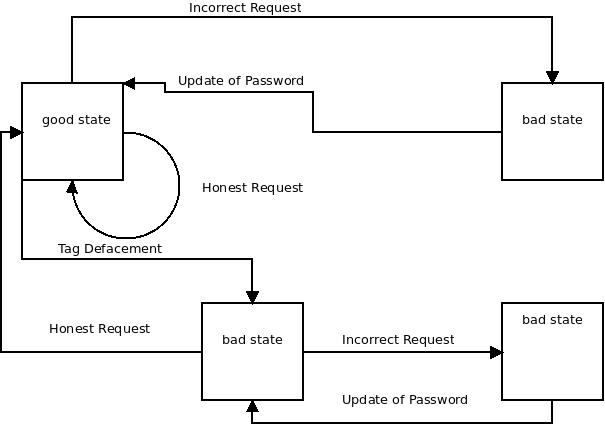
\psfig{file=Diagram1.jpg, height=2in, width=3in,}
\caption{State diagram for NFC tag protocol}
\end{figure}

Figure 1 contains the state diagram that we have to consider. This
diagram details the different ways that users can interact with the
system and also shows the requests that should be accepted and
rejected. There are three possible transitions between states. One is
an honest user interacting with the system, one is a malicious user
sending requests to the webserver directly, and the third is a
malicious user defacing the NFC tag.

From the description we can see that any request that moves the state
of the system from good to bad should be rejected because it is
malicious. Likewise, any request that moves the state from bad to good
should be accepted because it is an honest user.

\subsection{Argument for Correctness}
We will refer to Figure 1 and argue that the protocol that we have
described above guarantees all that we have described.

If the tag is in a good state i.e. it contains the next password that
the webserver is expecting, we can see that a sequence of honest users
will not result to a change to a bad state. Each user will read the
tag, submit the correct code to the server and then write the next
correct code to the tag. However, if one of these honest users drags
their phone away too fast, or if a malicious user comes in and defaces
the tag, we transition to a bad state. 

From this state, if an honest user comes in afterwards he will read
the wrong key and his request will get rejected. To deal with this, we
rely on the next honest request to fix our mistake. When a valid
request is accepted, the webserver goes back and checks to make sure
that the person that wrote that message to the tag gets their request
accepted as well. This way, even though it looks like an honest user
has to sacrifice a transaction to fix the state, we can actually roll
back their rejection and approve it provided that another valid
request comes in after them. It is worth noting that this only works
with the TPM because otherwise malicious users can just pass codes
around and confirm each other's requests.

Now that we have covered two of the states we can look at the cases
where requests get submitted from the web. If a request is submitted
from the web, we assume that it is not going to be the right password
since the chances of that happening are 1 in $2^{15}$ in our proof of
concept implementation, and can be arbitrarily lower if we choose a
longer cryptographically random key. If an incorrect request is sent
from any state, the transition is to a bad state and the webserver
will reject the request. After each transition to a bad state, the
state will then switch back to the one it was at previously after a
new password is generated. This guarantees that no web requests will
affect the protocol.

\subsection{Attack Prevention}
\begin{table}
\centering
\caption{Attack Prevention Table for Protocol 1}
\begin{tabular}{|c|c|l|} \hline
Attack&Protocol 1&Protocol 2\\ \hline
Bogus Submissions & YES & YES\\ \hline
Publicizing the Password& YES & YES\\ \hline
Multiple Scan& YES & YES\\ \hline
Tag Modification& YES & Vote Lost\\ \hline
Man In The Middle& YES & NO\\
\hline\end{tabular}
\end{table}


Please refer to Figure 2 to see how our protocol fares against
attacks. We can deal with bogus submissions as we argued with the
state model. Each password has one use, so publicizing it has no real
benefit. Multiple scans are disallowed by the web interface since the
phone has to submit an IMEI with each request, and even if that is
somehow avoided the requests are tied to the user scanning the tag so
they cannot be passed to a third party. Tag modification is fixable
with one honest user, and then that honest user can get their request
accepted when another honest user scans the tag after them. A MITM
attack can be prevented with the use of a TPM to hide the password
from the user, thus preventing him from forwarding it to anyone.

\subsection{Implementation}
We have implemented a proof of concept for this protocol, but since we
did not have a phone with a TPM on it we just worked under the
assumption that the passwords that the web interface gave the users
would be inaccessible. We tested the protocol with malicious and
honest requests and showed that the state transitions that we expected
were reproduceable in the real world.

\section{Protocol 2: Phone without TPM + Dumb Tag}
\subsection{Outline}
This is a quick rundown of the protocol:

\begin{enumerate}
\item The device reads the tag and the tag sends the device a code, $k$
\item The device sends the phone IMEI and $k$ to the webserver
\item The webserver checks $k$ against the key that it is expecting
\item The key matches so the webserver generates the next key, $l$, to write to the tag
\item The webserver records the fact that the device's request was accepted
\item The ACCEPTED message and $l$ are sent to the device 
\item The device writes $l$ to the tag so the next person can use it
\end{enumerate}

If you compare this protocol to the one that we just considered, you
can see that there are almost no differences. The protocol is
practically the same, but now we have relaxed the requirement of an
on-phone TPM. This is very significant, because it means that
malicious users have unfettered access to the keys sent to them
by the webserver and tag. 

\subsection{Attack Prevention}
For this protocol we cannot really show correctness because we don't
actually have it. What we do have is a very good system for minimizing
the possible damage that the attacks can do. 

Please refer to Figure 2 to see how our protocol fares against
attacks. We can deal with bogus submissions the same way that we did
in the first protocol. In this regard, nothing has changed. False
requests have no real impact. Each password has one use, so
publicizing it has no real benefit. Multiple scans are disallowed by
the web interface since the phone has to submit an IMEI with each
request, and even if that is somehow avoided the requests are tied to
the user scanning the tag so they cannot be passed to a third party en
masse. What can happen is that it can be passed a single time (a man
in the middle attack that we will discuss below). Tag modification is
fixable with one honest user, but in this case we cannot roll the log
back and re-accept the user that fixed the tag. This is because we
have no guarantee that two malicious users won't get together and
confirm each other's requests. All it takes in this scenario is for
one to submit a faulty request, and then pass the new password that he
is given to his friend. That way both of them now have valid entries
in the log. Because of this, we have to turn this feature off and deal
with the fact that every time a malicious user modifies the tag, we
will use one honest user's submission. We can implement a clever
mechanism to deal with this to prevent it from becoming a real
problem. Unfortunately, a MITM attack has full reign under this
protocol because we have no means to prevent people from passing their
keys to other users. We argue that this isn't really all that bad
considering the fact that at least someone has to be at the location
and that MITM requires some coordination because it has to be
completed before another user walks up to the tag and scans it. Since
there isn't a good way to prevent MITM with a dumb tag and a phone
that can't shield information from the user, we will focus on cutting
down the number of malicious users in the system in general to lessen
their effect on the good users.

\subsection{Reputation System}
A reputation system seems like the obvious choice for this
scenario. If users have to authenticate to the webserver and if their
acceptances and rejections are tied to their account, it makes it
harder for repeat offenders to affect the system. Privacy is a
concern, but in this case the only thing that the reputation system
has to tie to the user is the number of times their requests have been
accepted or rejected. We do not need to know where exactly these
requests came from, so it can't really be tied to a real identity.

The way that we propose to do the reputation system involves adding
certain numbers of strikes to users for actions that are possibly
malicious. These actions are associated with being one of the people
around the transitions to the bad states in the state diagram in
Figure 1. If the same user is seen transitioning the system to a bad
state it is safe to assume that he is a malicious user, and then he
can be banned from the system. This prevents outlying malicious users
from flooding the system with bad requests and repeatedly defacing the
tag, which as we covered above, results in the loss of good votes.

Since it is hard to tell how a reputation system will work without
trying it first, we ran several simulations.

\subsection{Simulations}
We ran the simulations in a similar way. We had several threads for
malicious users, and a thread for honest users. We ran each simulation
for 30 simulated days and collected data at the end for the number of
good requests that were dropped from the log. The variables that we
tweaked in the simulation were the ratio of malicious users to good
users and the number of requests issued to the service. These
variables were reflected in the timing of the threads. For example, in
a system that is very popular and with a small fraction of malicious
users we have the good thread printing often, and the malicious
threads printing rarely. We then parse the resulting logfile and
compare the number of confirmed accepted requests to the expected
number. We return the result as a percentage.

When we ran the simulations without a reputation system, the number of
honest user requests that was dropped was pretty much equal to the
number of tag defacements that occurred during the simulation. This
makes intuitive sense because every time a tag is brought out of sync,
a good user has to sacrifice a vote in order to sync it up again. With
the addition of a reputation system, however, the numbers that we got
were always lower than without the system. Especially when the
malicious users were small in number, they got weeded out of the
system fairly quickly. This bodes well for the system because since
the users have to be at the physical location, it prevents several
users that live or work in the vicinity from strongly affecting honest
users.

We did not take into account malicious requests sent from the web
because they would not affect our protocol either way. With the
reputation system however, they would actually improve results and
allow us to stop malicious users even faster. Please refer to Table 2
for the results of the simulations:

\begin{table}
\centering
\caption{Simulations of Protocol 2}
\begin{tabular}{|c|c|c|l|} \hline
Total Requests&Bad Users&Reputation Enabled&\% Dropped\\ \hline
3058&100&NO&10.16\\ \hline
2976&100&YES&9.22\\ \hline
2187&10&YES&1.72\\ \hline
\hline\end{tabular}
\end{table}

\section{Results}
We can see from the results of the simulation that the second protocol
works fairly well even without a TPM. This is the lowest cost solution
that we can hope for, and with the addition of a reputation system we
can have a fairly stable system that is relatively resistant to
attacks by malicious users.

Of course the better alternative is to use the first protocol where we
dont have to bother with a reputation system and don't have to worry
about MITM attacks, but no commercial phone currently has a TPM on
it. It might be a reasonable thing to expect in the future since a lot
of laptops are currently being released with TPMs built in, but it is
not a reasonable thing to expect in the next year.

\section{Further Research}
This paper focused heavily on the webserver and the device side of the
problem. If we consider tags that have timing code or can
cryptographically sign messages we can consider other possible
solutions. Dumb tags are the most common form right now and will
definitely be cheaper than the smarter alternative, so any protocol
that assumes a smart tag has to look to the future in terms of
real-world implementation.


\end{document}
